\documentclass[BSP,english,oneside]{ntnuthesis/ntnubachelorthesis}

\usepackage{csvsimple}
\usepackage{booktabs}
\usepackage{import} % Used for import from folders.
\usepackage{mathtools}
\usepackage[miktex]{gnuplottex}

\usepackage[T1]{fontenc}
\usepackage[utf8]{inputenc}
\usepackage{lmodern}
\usepackage[miktex]{gnuplottex}
\usepackage{graphicx}

\usepackage[binary-units=true]{siunitx}
\DeclareSIUnit\year{yr}

\import{../latex_utility/}{listing_cpp_syntax.tex}
\import{../latex_utility/}{pt_commands.tex}

%\renewcommand{\comment}[1]{\textcolor{blue}{\emph{#1}}}  %% use of the colour and you can see how to use commands with parts
\newcommand{\com}[1]{{\color{red}#1}} % supervisor comment
%\renewcommand{\com}[1]{} %remove starting % to remove supervisor comments
% This will appear in text \com{Lecuters comment} and be visible unless you uncomment
% the renewcommand line.

\newcommand{\todo}[1]{{\color{cyan}\lbrack todo: #1\rbrack}\\} % items to do
%\renewcommand{\todo}[1]{} %remove starting % to remove items to do

\newcommand{\n}[1]{{\color{blue}#1}} % other comment
%\renewcommand{\n}[1]{} %remove starting % to remove notes

\newcommand{\dn}[1]{} % add the dn to a note to say that you have finished with it.

% To use when just doing a regular section reference, if more custom wording is needed,
% the footnote must be set up manually
\newcommand{\secref}[1]{\footnote{See section \ref{#1}}}

\newcounter{ptrequirements}
\newcommand{\requirement}[2]{\begin{quote}\refstepcounter{ptrequirements}\textbf{Requirement \theptrequirements: #1 \label{#2}}\end{quote}}
\newcommand{\reqref}[1]{\footnote{Requirement \ref{#1}.}}
\newcommand{\reqcomment}[1]{\emph{Comment: #1}}

\def \gnuplotterminal {pdf}
%\newcommand{}{pdf}

\begin{document}

\subimport{inc/}{thesis_data.tex}

\makefrontpages

\subimport{inc/}{preface.tex}

\tableofcontents
\listoffigures
\listoftables

\todo{Add note, entities and actors are the same thing}
\todo{Add note that user and programmer are the same thing!}

\subimport{inc/}{introduction.tex}
\subimport{inc/}{requirements.tex}
\subimport{inc/}{technical.tex}
\subimport{inc/}{measurements.tex}
\subimport{inc/}{benchmarking.tex}
\subimport{inc/}{discussion.tex}
\subimport{inc/}{future_work.tex}
\subimport{inc/}{process.tex}
\subimport{inc/}{conclusion.tex}

\bibliographystyle{ntnuthesis/ntnubachelorthesis}
\bibliography{inc/thesis}

\todo{Add issue tracking and estimation section to process}
\todo{Download newest version of thesis template}


\appendix %after this line all chapters will have leters instead of numbers
%\chapter{Test Case Plan}
%\chapter{Design Document}
%\chapter{Technical Specification}
%\chapter{Project Plan}
%\chapter{Scrum Plans}
%\chapter{Daily Scrum Logs}
%\chapter{Stakeholder Meetings}
%\chapter{Supervisor Meetings}
%\chapter{Sprint Retrospectives}
%\chapter{Group Rules}
%\chapter{Benchmark Data}
%\chapter{Stakeholder Contract}
%\chapter{Code}

\todo{Add to appendix!}
\begin{figure}
    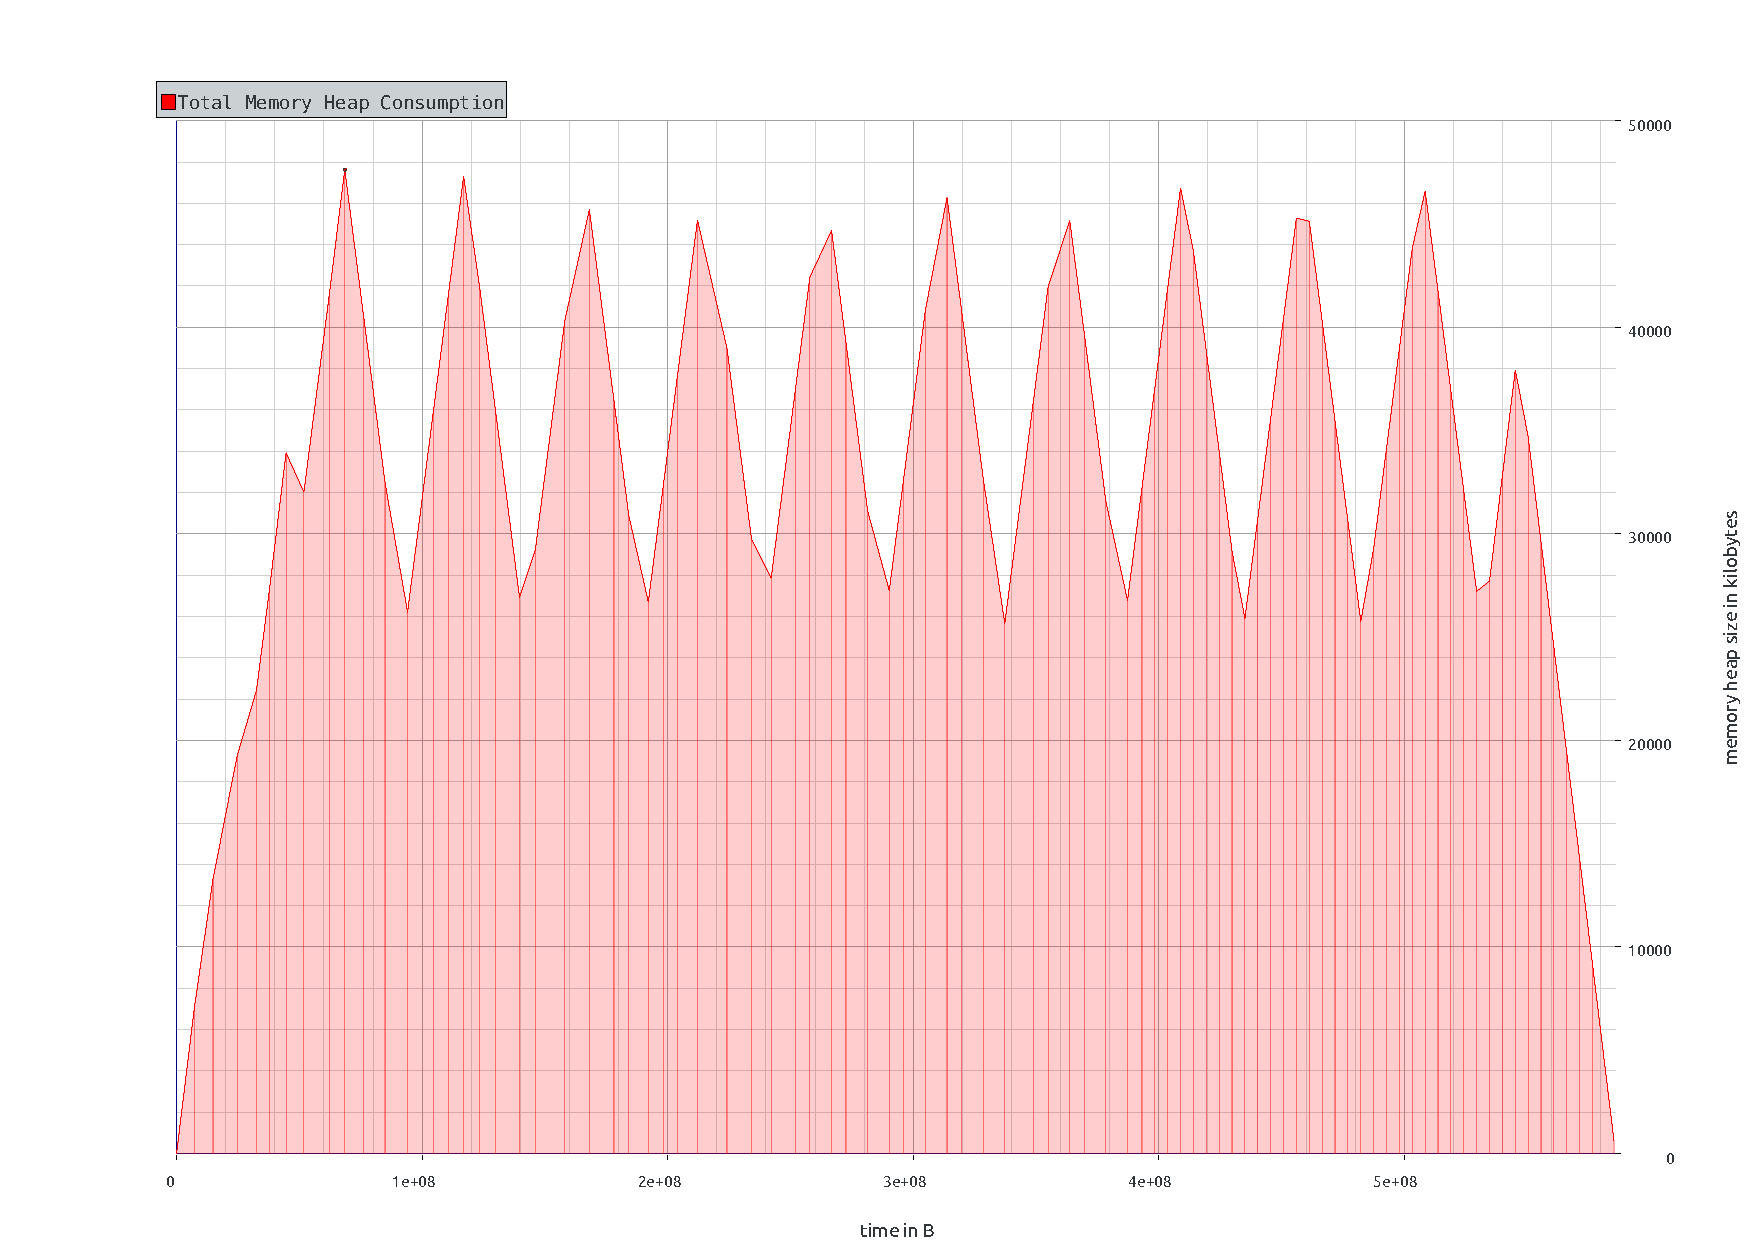
\includegraphics[scale=0.5]{benchmark_results/fast_spawn/ecs_massif_deletes_10.pdf}
    \caption{Fast spawning memory usage, NOX ECS}
    \label{fig:fast_spawning_memory_usage_nox_ecs}
\end{figure}

\begin{figure}
    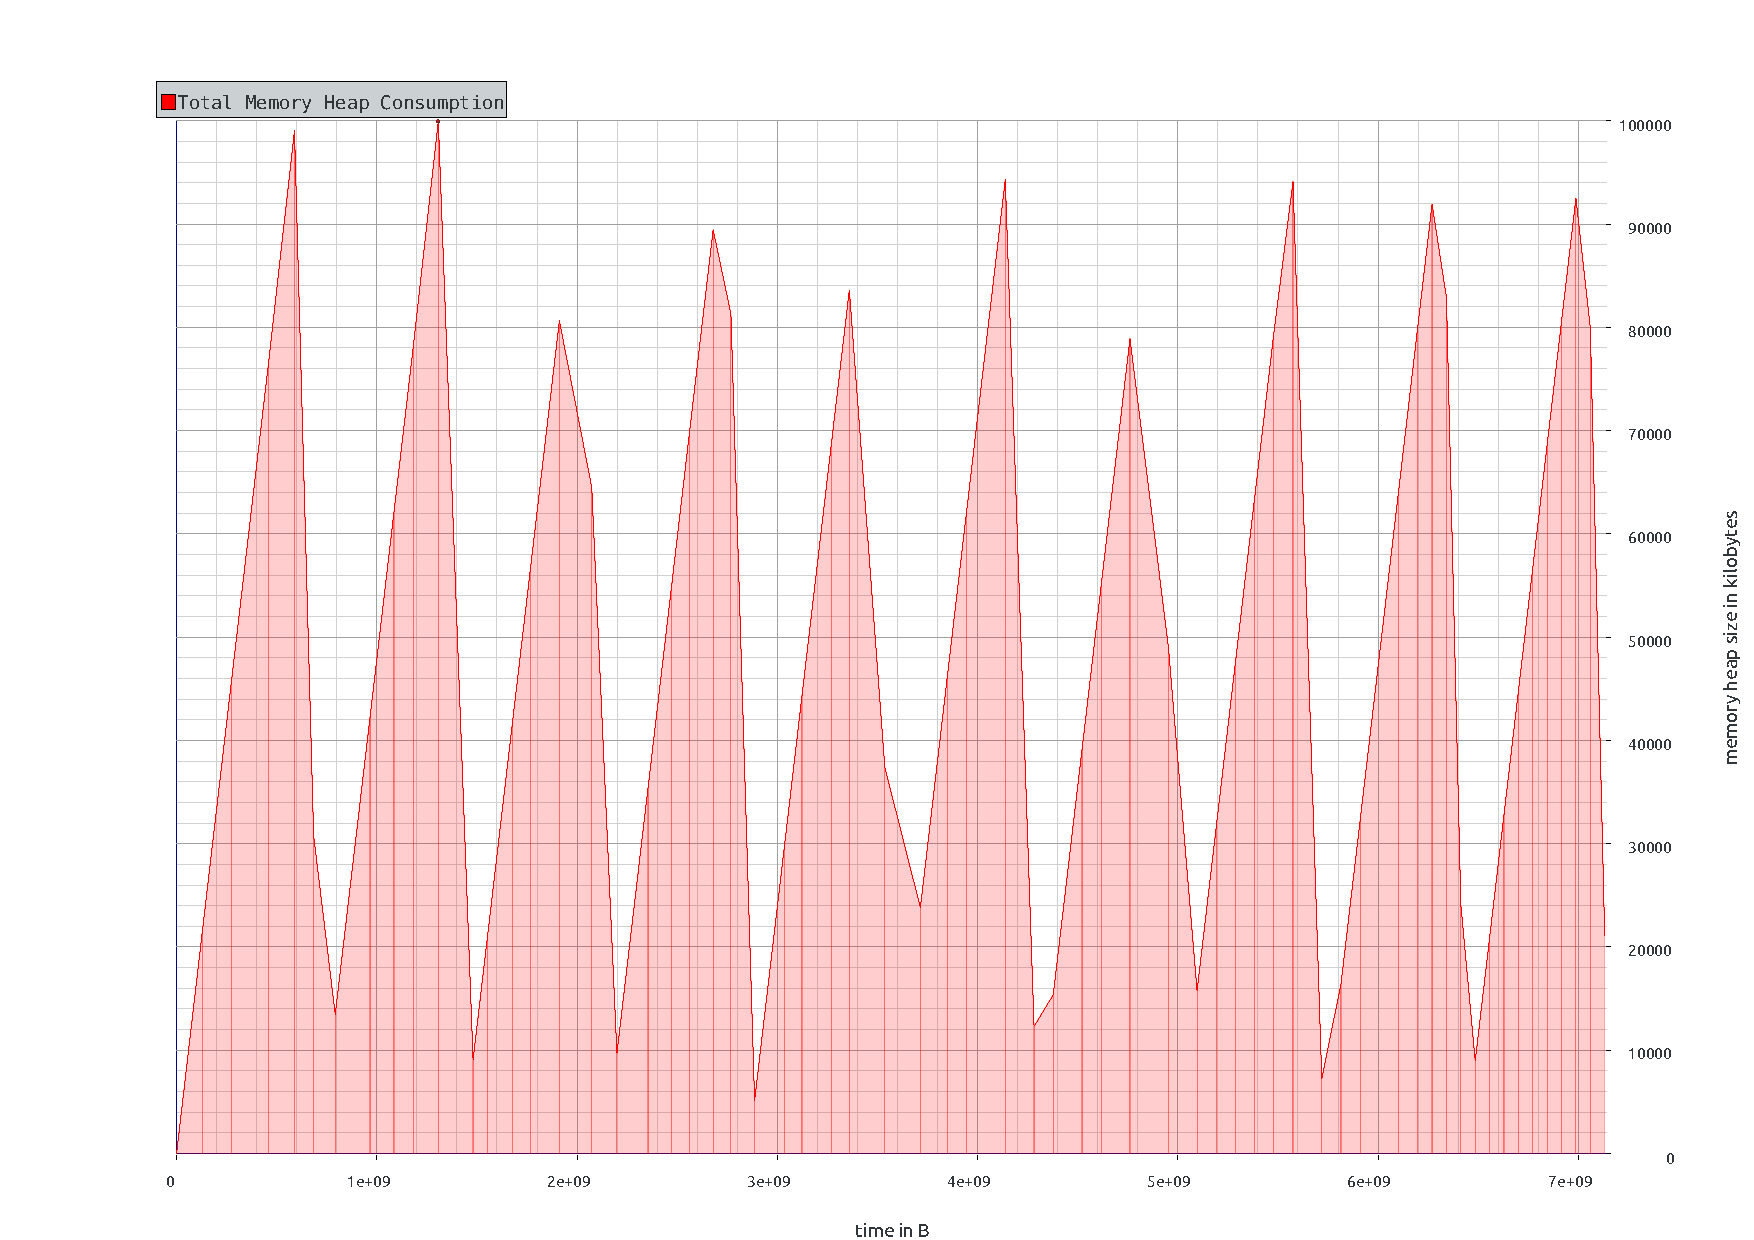
\includegraphics[scale=0.5]{benchmark_results/fast_spawn/nox_massif_deletes_10.pdf}
    \caption{Fast spawning memory usage, NOX Actor}
    \label{fig:fast_spawning_memory_usage_nox_actor}
\end{figure}



Justify that we are doing just one test properly.


Do the rest of the tests before the presentation.
When in doubt do citations.
Ok that the test is not representative for our best case.

The optimization toggles are their own tests, and having them be different is ok.'


Write:
Should have timed right before update has started, so we didnt get the execution layer overhead, etc.

Uniqueptr test case not entirely correct, as it will also update entities that are hibernating etc,
however it is not relevant for that test case, as we don't have any deactivate components.

Give short explanation on how to see the cachegrind stuff.

\end{document}

% More explanations in technical, not requirements.
% Do reference back in time, not forward.
% Cite books, should be enough for the standard.
% Only code snipets in the thesis, no need to include all files.
% Explain SFINAE
% Footnotes for "fire and forget" comments
% Oversight that we are not doing the sparse outer array thingy.
